\providecommand{\main}{../../..}
\documentclass[\main/main.tex]{subfiles}
\begin{document}

\subsection{Esercizio 6}
Si consideri un problema di teoria delle decisioni con 3 soluzioni alternative, indicate da $x_1$, $x_2$ e $x_3$ e 2 stati di natura, indicati da $\omega_1$ e $\omega_2$.

Le seguenti tabelle riportano la funzione $f(x, \omega)$ che rappresenta dei benefici e le probabilità congiunte $p(\omega, y)$ degli stati di natura e dei risultati di un esperimento che può avere 2 esiti, indicati da $y_1$ e $y_2$. Qual è la strategia ottima?

\begin{figure}
  \begin{subfigure}{0.49\textwidth}
    \begin{table}
      \begin{tabular}{|L|L|L|}
        \hline
        f(x, \omega) & \omega_1 & \omega_2 \\
        \hline
        x_1          & 40       & 40       \\
        \hline
        x_2          & 100      & 0        \\
        \hline
        x_3          & 10       & 80       \\
        \hline
      \end{tabular}
    \end{table}
  \end{subfigure}
  \begin{subfigure}{0.49\textwidth}
    \begin{table}
      \begin{tabular}{|L|L|L|}
        \hline
        p(\omega, y) & \omega_1 & \omega_2 \\
        \hline
        y_1          & 0.1      & 0.4      \\
        \hline
        y_2          & 0.3      & 0.2      \\
        \hline
      \end{tabular}
    \end{table}
  \end{subfigure}
\end{figure}

\subsection{Soluzione esercizio 6}
\begin{figure}
  \begin{tikzpicture}
    \Tree[.root
    [.\text{faccio esperimento}
    [.$0.5$
      [.$y_1$
          [.$x_1$
              [.$0.2$
                  [.$\w_1$
                      [.$40$ ]
                    ]
                ]
                [.$0.8$
                  [.$\w_2$
                      [.$40$ ]
                    ]
                ]
            ]
            [.$x_2$
              [.$0.2$
                  [.$\w_1$
                      [.$100$ ]
                    ]
                ]
                [.$0.8$
                  [.$\w_2$
                      [.$0$ ]
                    ]
                ]
            ]
            [.$x_3$
              [.$0.2$
                  [.$\w_1$
                      [.$10$ ]
                    ]
                ]
                [.$0.8$
                  [.$\w_2$
                      [.$80$ ]
                    ]
                ]
            ]
        ]
    ]
    [.$0.5$
      [.$y_2$
          [.$x_1$
              [.$0.6$
                  [.$\w_1$
                      [.$40$ ]
                    ]
                ]
                [.$0.4$
                  [.$\w_2$
                      [.$40$ ]
                    ]
                ]
            ]
            [.$x_2$
              [.$0.6$
                  [.$\w_1$
                      [.$100$ ]
                    ]
                ]
                [.$0.4$
                  [.$\w_2$
                      [.$0$ ]
                    ]
                ]
            ]
            [.$x_3$
              [.$0.6$
                  [.$\w_1$
                      [.$10$ ]
                    ]
                ]
                [.$0.4$
                  [.$\w_2$
                      [.$80$ ]
                    ]
                ]
            ]
        ]
    ]
    ]
    [.\text{non faccio esperimento}
    [.$x_1$
      [.$0.4$
          [.$\w_1$
              [.$40$ ]
            ]
        ]
        [.$0.6$
          [.$\w_2$
              [.$40$ ]
            ]
        ]
    ]
    [.$x_2$
      [.$0.4$
          [.$\w_1$
              [.$100$ ]
            ]
        ]
        [.$0.6$
          [.$\w_2$
              [.$0$ ]
            ]
        ]
    ]
    [.$x_3$
      [.$0.4$
          [.$\w_1$
              [.$10$ ]
            ]
        ]
        [.$0.6$
          [.$\w_2$
              [.$80$ ]
            ]
        ]
    ]
    ]
    ]
  \end{tikzpicture}
\end{figure}

\begin{figure}
  \begin{tikzpicture}
    \Tree[.root
    [.\text{faccio esperimento}
    [.$0.5$
      [.$y_1$
          [.$x_1$
              [.$40$ ]
            ]
            [.$x_2$
              [.$20$ ]
            ]
            [.$x_3$
              [.$66$ ]
            ]
        ]
    ]
    [.$0.5$
      [.$y_2$
          [.$x_1$
              [.$40$ ]
            ]
            [.$x_2$
              [.$60$ ]
            ]
            [.$x_3$
              [.$38$ ]
            ]
        ]
    ]
    ]
    [.\text{non faccio esperimento}
    [.$x_1$
      [.$40$ ]
    ]
    [.$x_2$
      [.$40$ ]
    ]
    [.$x_3$
      [.$52$ ]
    ]
    ]
    ]
  \end{tikzpicture}
\end{figure}

Eseguendo l'esperimento la scelta migliore risulta essere $x_3$, scelta che mantiene l'ottimalità anche quando si sceglie di non eseguire l'esperimento.

\end{document}
